\documentclass[12pt]{article}

%----------------------Autor y fecha----------------------




%------------------------Paquetes-------------------------

\usepackage{graphicx}			% Gráficos
\usepackage[utf8]{inputenc}		% Codificación
\usepackage[spanish]{babel}		% Idioma
\usepackage{lastpage}
\usepackage{dcolumn}			% Tablas
\usepackage{enumitem}			% Listas
\usepackage{bm}					% Negrita en ecuaciones
%\usepackage{pstricks}			% Arboles
%\usepackage{pst-tree}			% 
\usepackage{amsmath,caption,booktabs}
\usepackage{amssymb}




\graphicspath{ {./Imagenes/} }
%---------------------------------------------------------

%------------------------Márgenes-------------------------

\usepackage{vmargin}
\setpapersize{A4}
\setmargins{3cm}	% margen izquierdo
{1.25cm}			% margen superior
{16.5cm}			% anchura del texto
{24.2cm}			% altura del texto
{18pt}				% altura de los encabezados
{1cm}				% espacio entre el texto y los encabezados
{10pt}				% altura del pie de página
{2cm}				% espacio entre el texto y el pie de página
%---------------------------------------------------------

%-----------Tamaño de Encabezado y Pie de pagina----------

\usepackage{fancyhdr}						% Paquete

\setlength{\headwidth}{\textwidth}
\setlength{\headheight}{28pt}
\setlength{\footskip}{1cm}
\renewcommand{\headrulewidth}{0.4pt}
\renewcommand{\footrulewidth}{1pt}

%---------------------------------------------------------

%---------------------Diseño Encabezado-------------------

\fancyhead[L]{
\includegraphics[height=.5cm]{./logos/UTN-FRSF.jpg}}
\fancyhead[R]{\textsf{\Large{Ingeniería en Sistemas de Información}}}
%---------------------------------------------------------

%--------------------Diseño Pié de pagina-----------------


\fancyfoot[R] {\thepage \textnormal{ de} \pageref{LastPage}}
\fancyfoot[L]{Grupo 4A:\scriptsize{\textit{ Bode, Busso, Ferraro Trivelli, Storani}}}
\fancyfoot[C]{2019}
%---------------------------------------------------------



%\renewcommand{\familydefault}{\sfdefault}	% Cambio de fuente por defecto

\pagestyle{empty}							% Estilo de página (Habilita los encabezados y pié de página)

\title{Correcciones Mockups -- TP Diseño de Sistemas}
\author{Grupo 4A}
\date{24 de agosto de 2019}



\begin{document}
		
\begin{titlepage}
\pagestyle{empty}
\center
\pagestyle{empty}
\maketitle
\newpage
\end{titlepage}

\pagestyle{fancy}

%%%%%%%%%%%%%%%%%%%%%%%
%%%%%%        CASO DE USO 1         %%%%%
%%%%%%%%%%%%%%%%%%%%%%%
\vfill
\begin{figure}[h!]
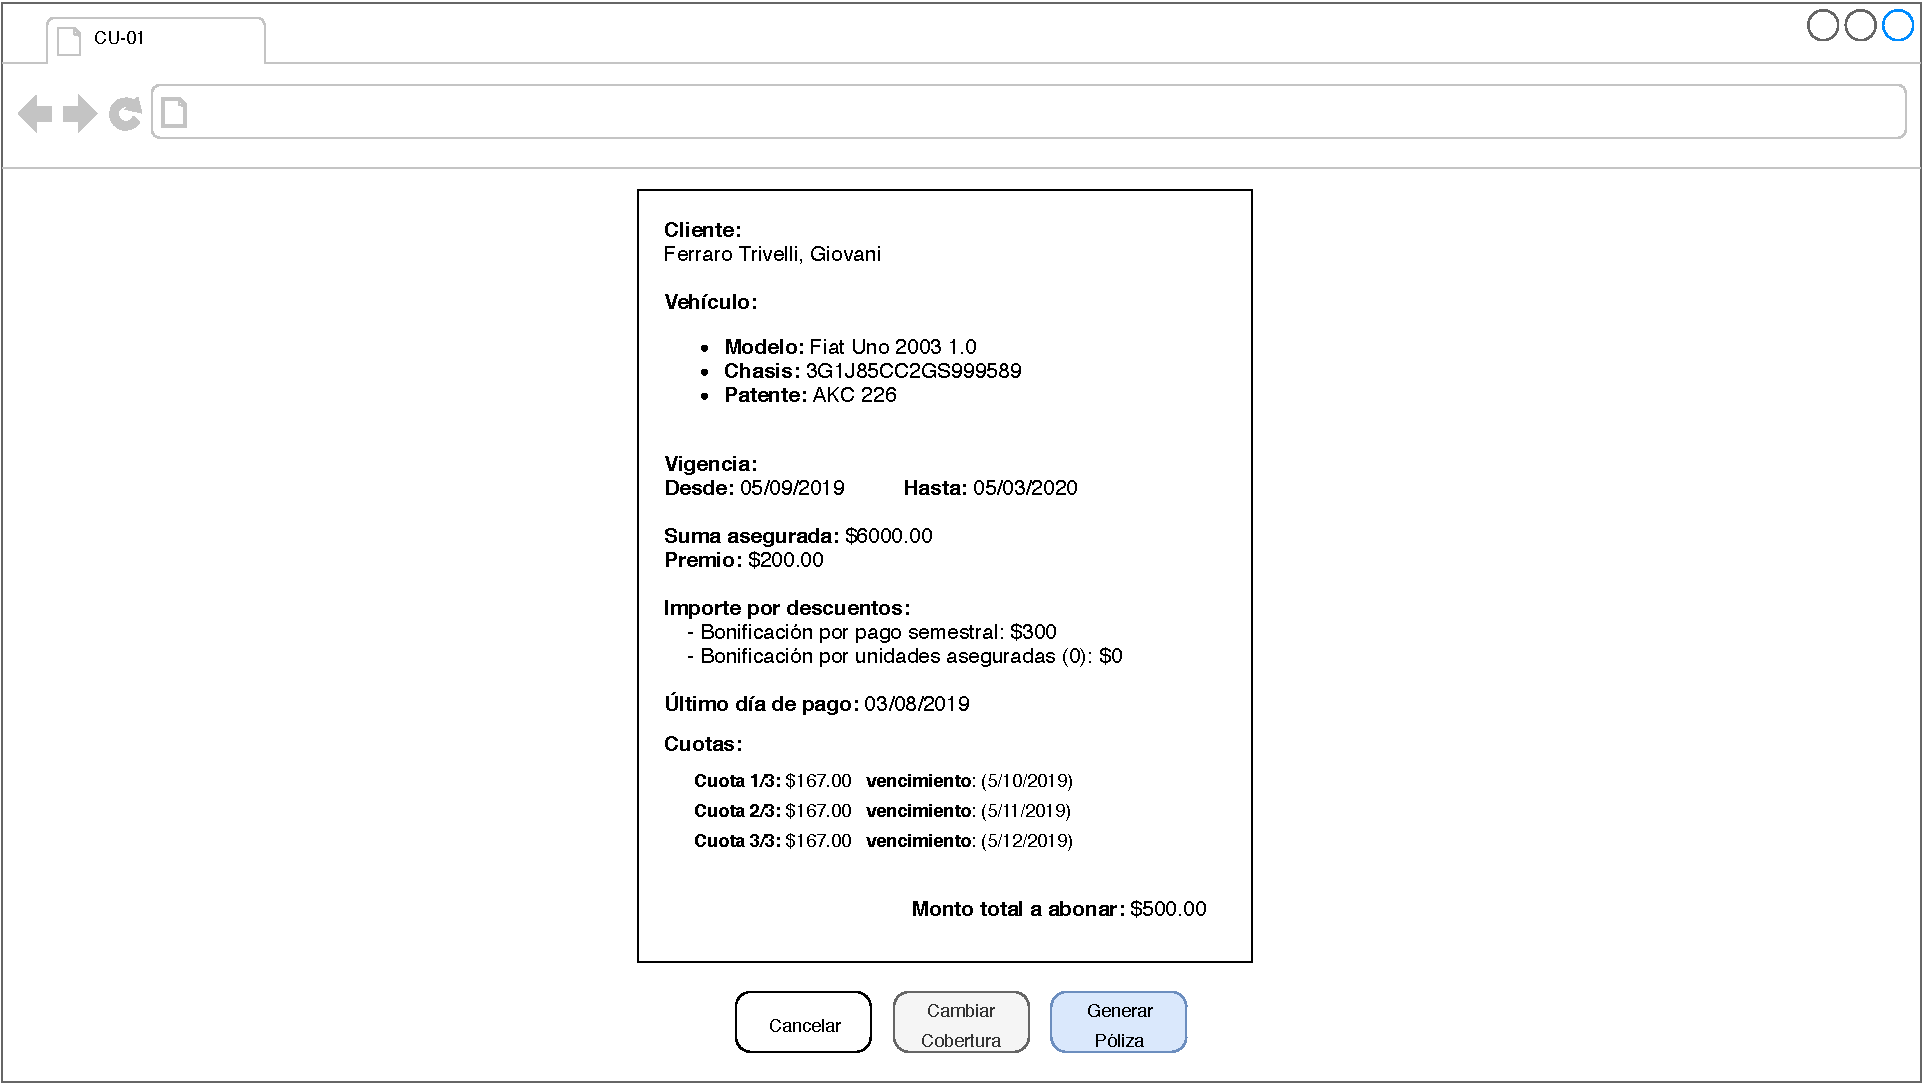
\includegraphics[width=\textwidth]{CU1/CU-017.pdf}
\caption{Caso de uso 1 (flujo principal)}
\end{figure}
\vfill



\vfill
\begin{figure}[h!]
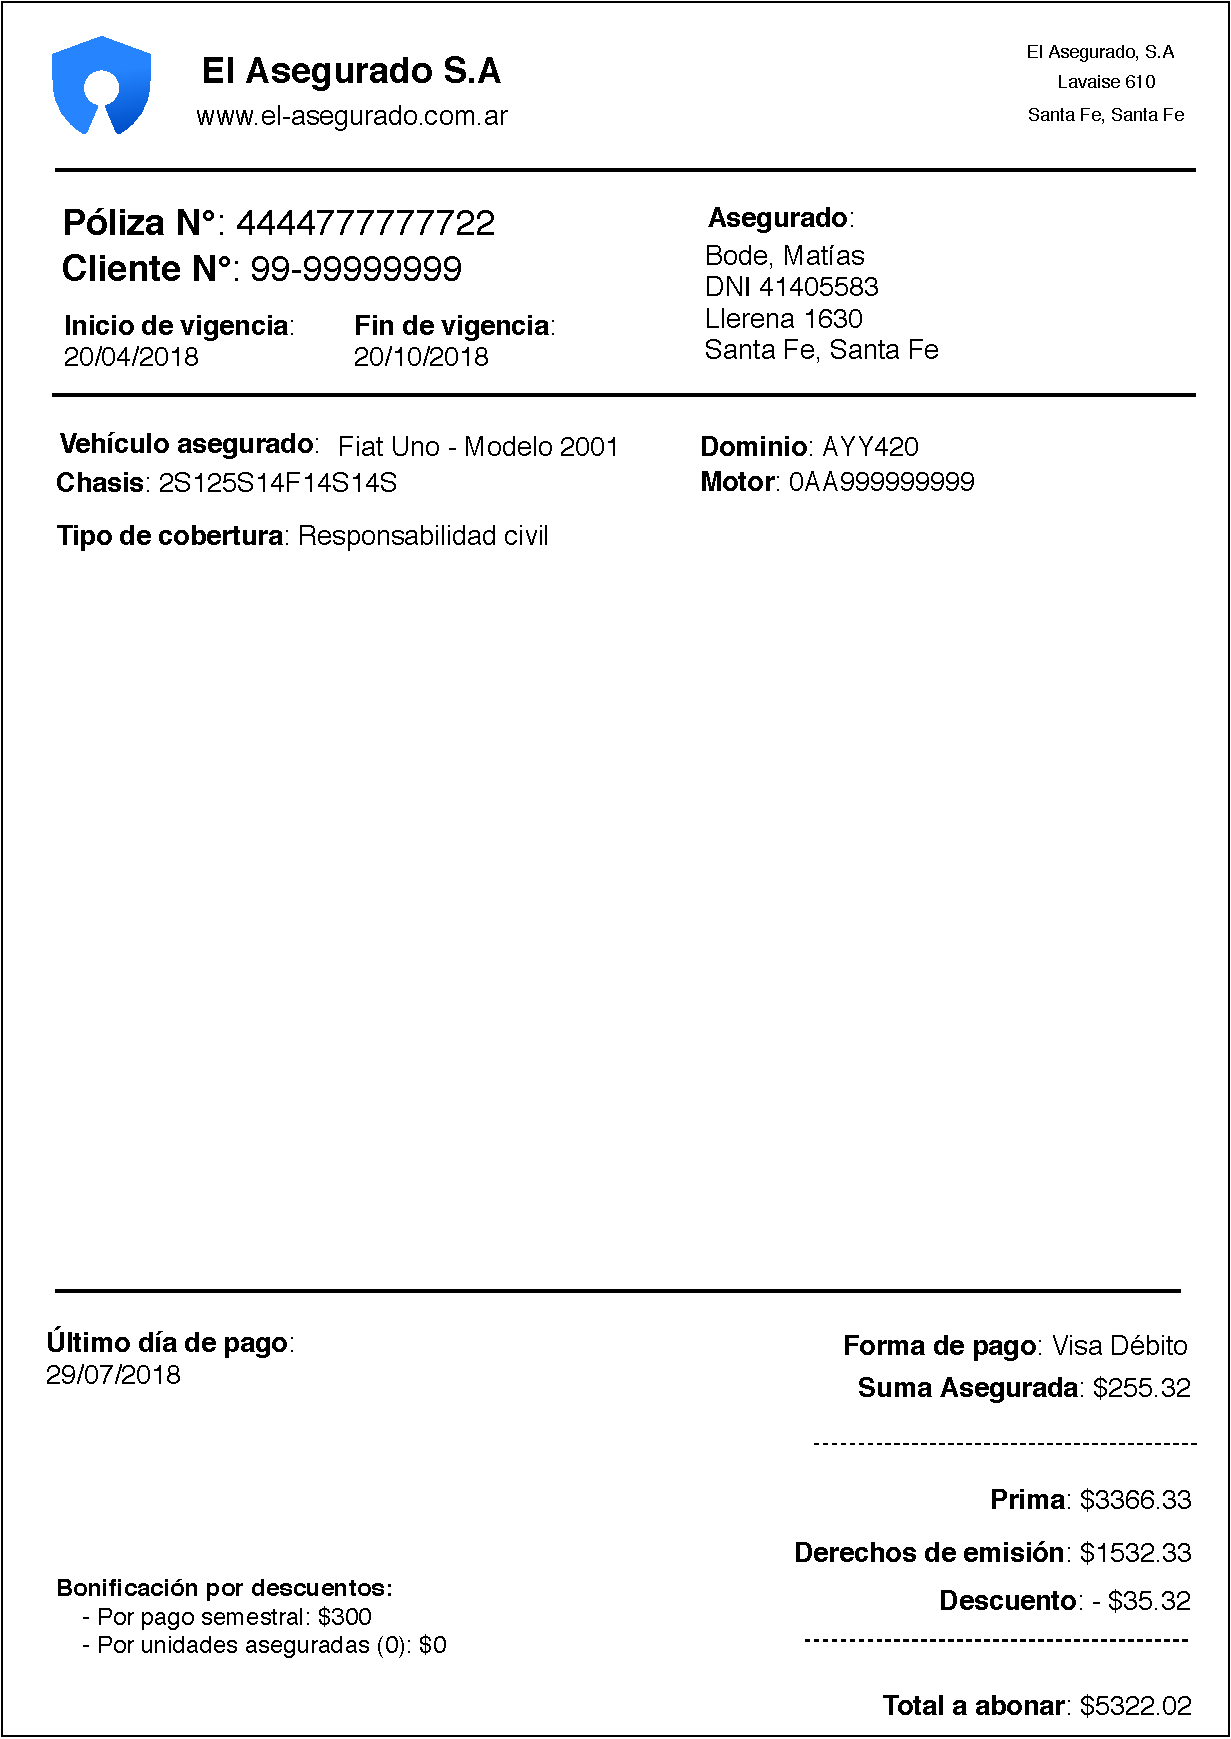
\includegraphics[width=\textwidth]{CU11/CU-111.pdf}
\caption{Caso de uso 11 (flujo principal)}
\end{figure}
\vfill


\vfill
\begin{figure}[h!]
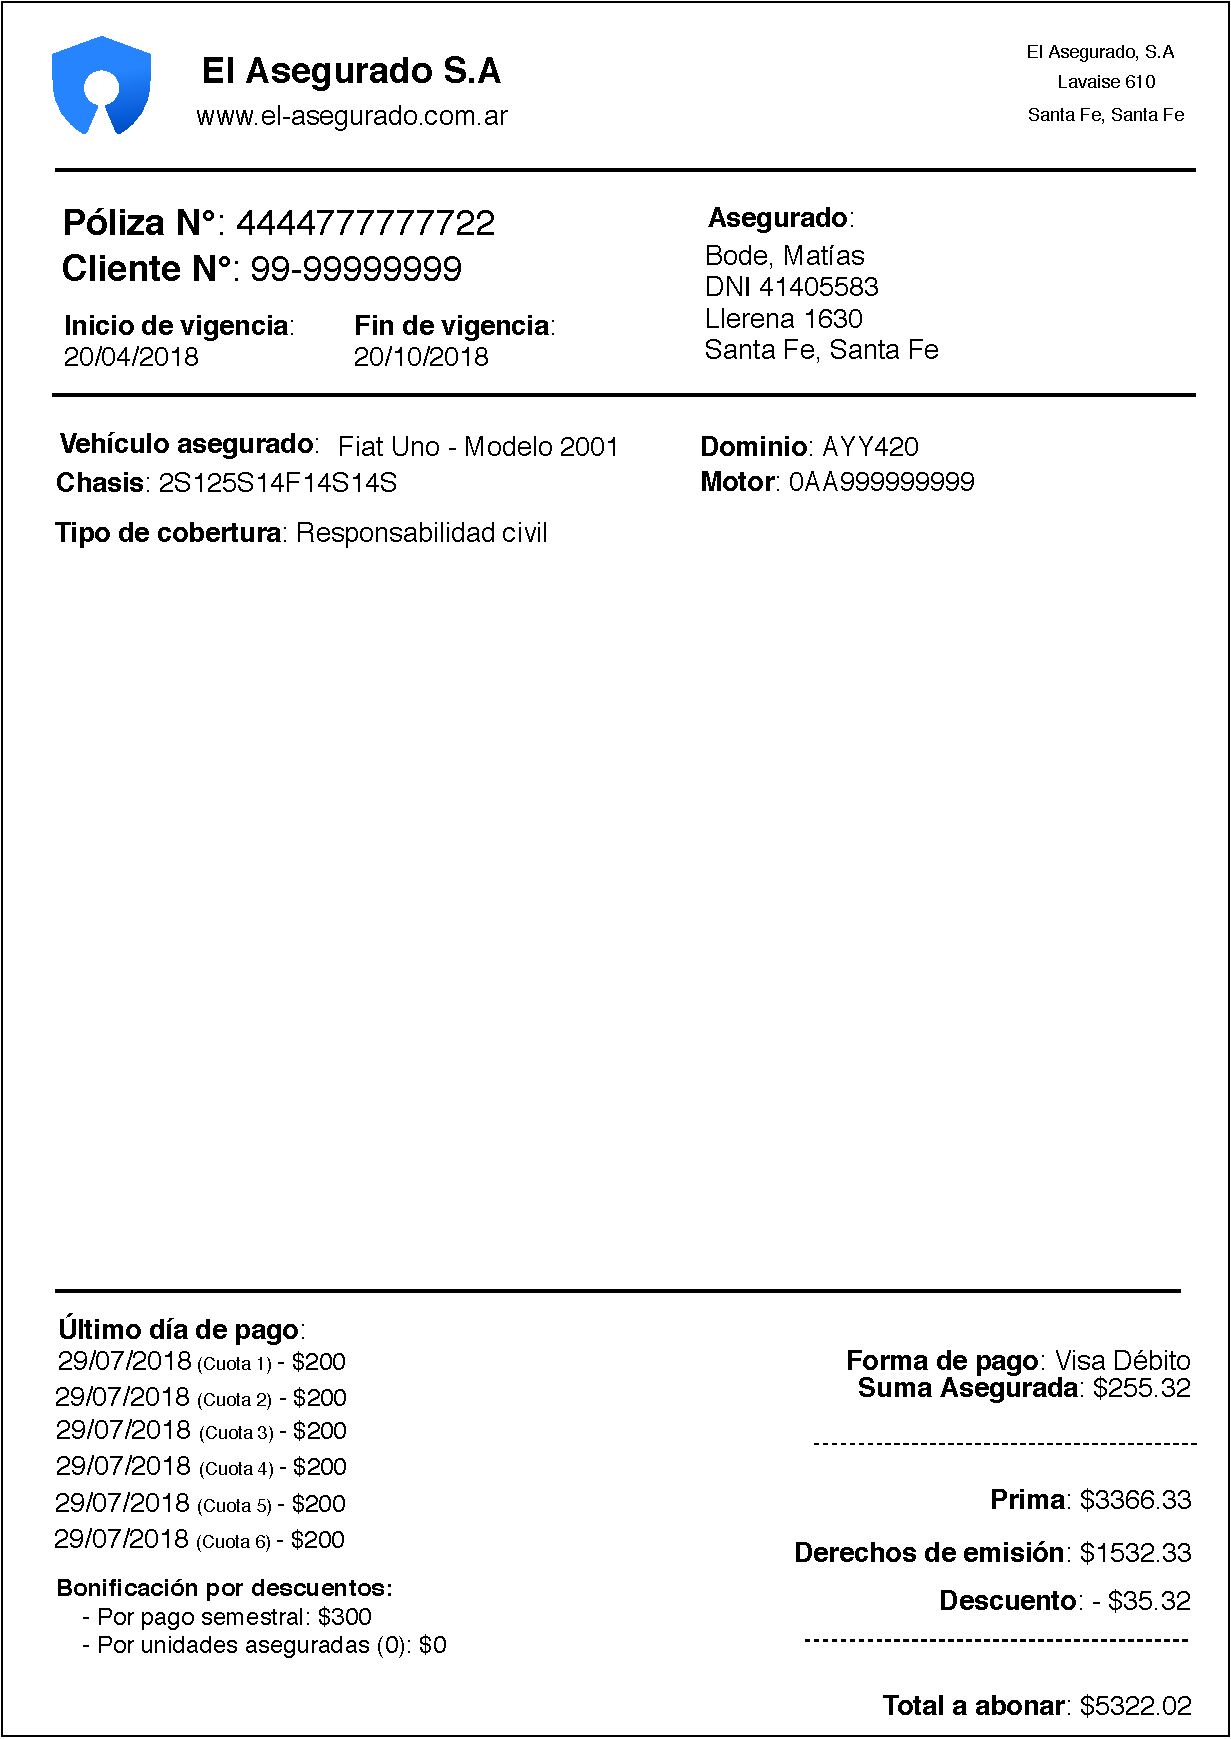
\includegraphics[width=\textwidth]{CU11/CU-112.pdf}
\caption{Caso de uso 11 (flujo principal)}
\end{figure}
\vfill


\vfill
\begin{figure}[h!]
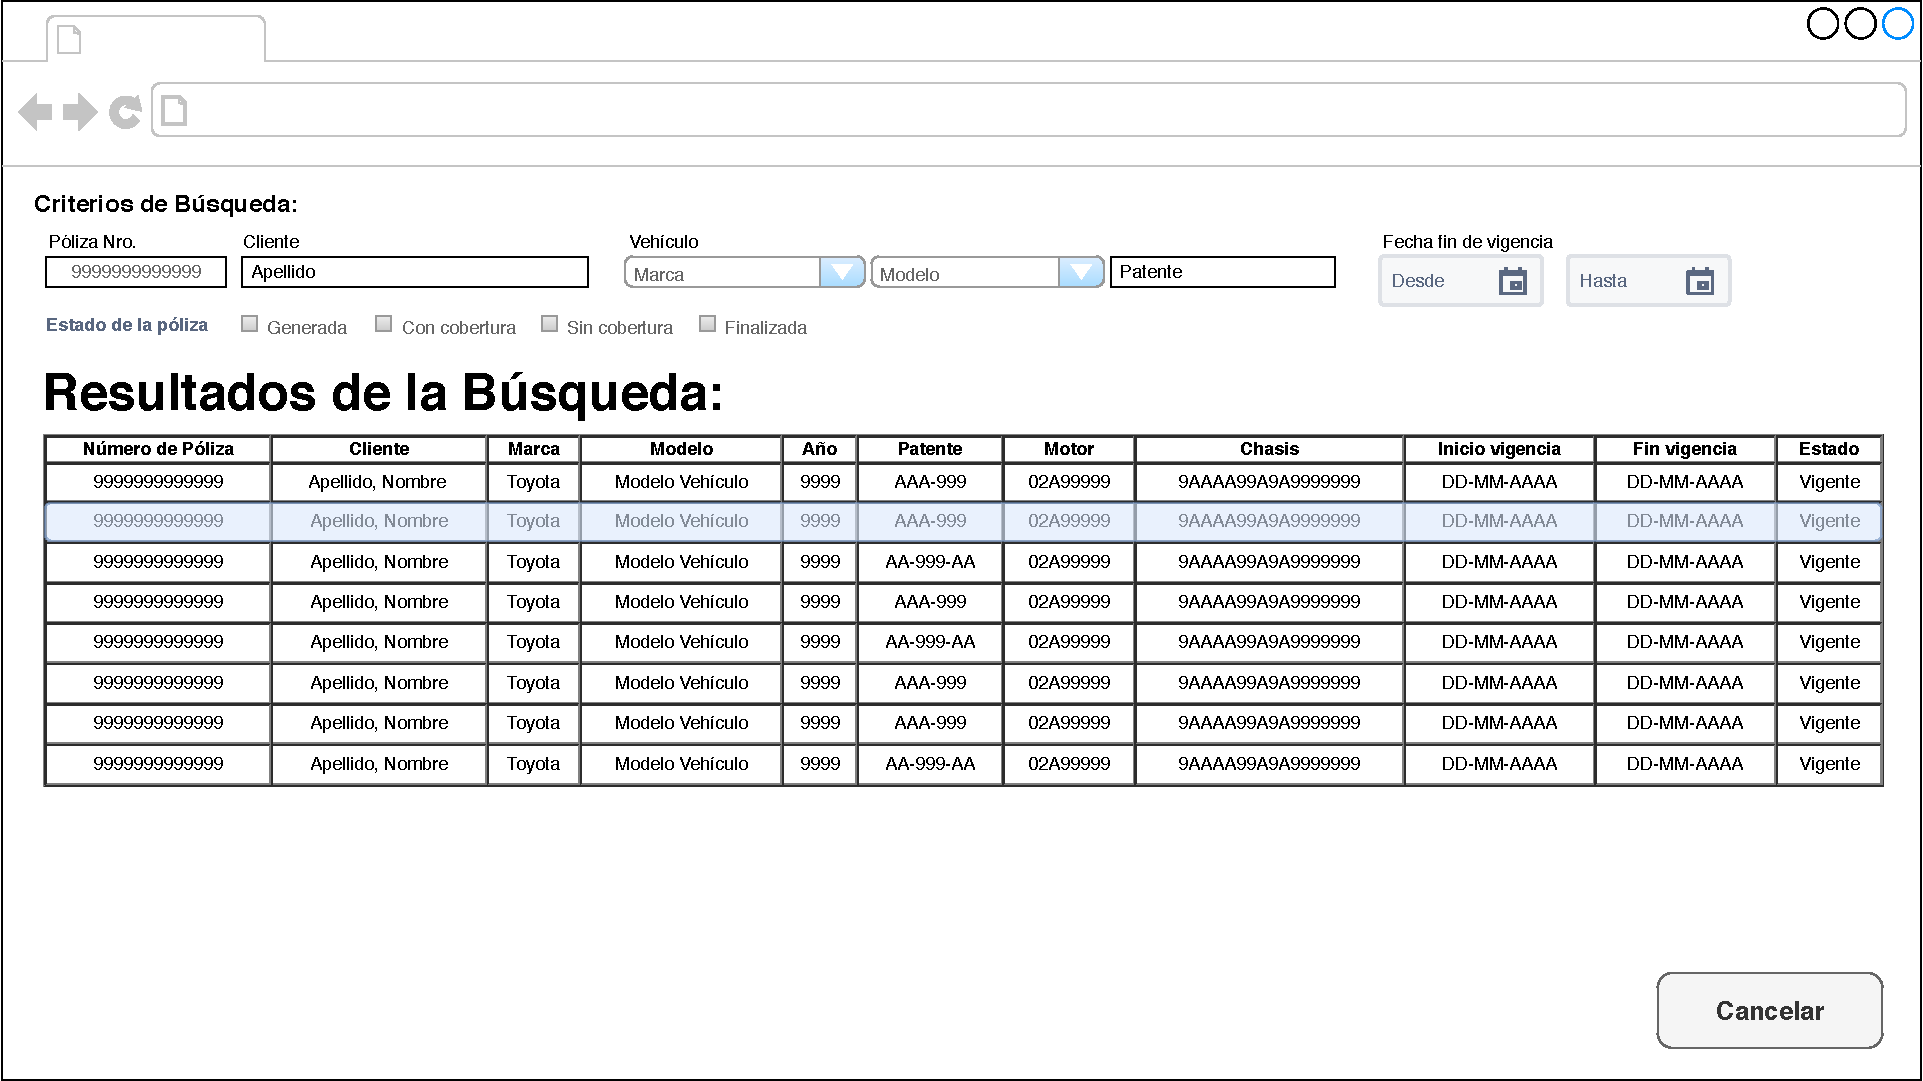
\includegraphics[width=\textwidth]{CU2/CU-024.pdf}
\caption{Caso de uso 2 (flujo principal)}
\end{figure}
\vfill

\end{document} 
